\documentclass{standalone}
\usepackage{tikz}
\usetikzlibrary{patterns, positioning}

\begin{document}
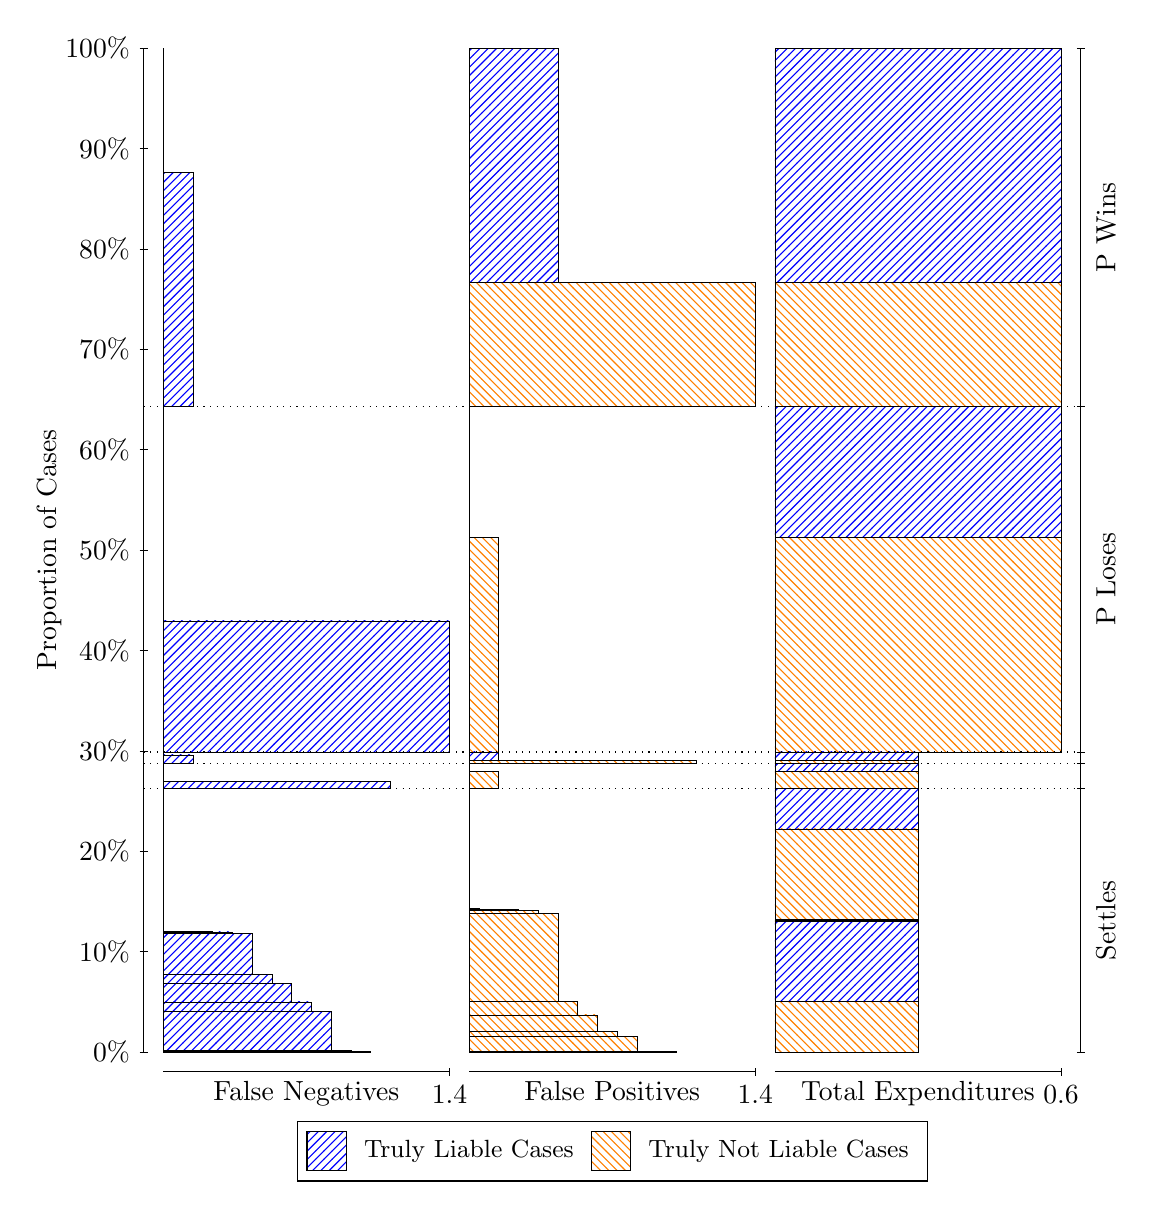
\begin{tikzpicture}
\draw[black, very thin] (1.5,1.75) -- (1.5,14.5);
\node[rotate=90, anchor=center] at (0.3, 8.125) {Proportion of Cases};
\draw[black, very thin] (1.45,1.75) -- (1.55,1.75);
\node[anchor=east] at (1.45, 1.75) {0\%};
\draw[black, very thin] (1.45,3.025) -- (1.55,3.025);
\node[anchor=east] at (1.45, 3.025) {10\%};
\draw[black, very thin] (1.45,4.3) -- (1.55,4.3);
\node[anchor=east] at (1.45, 4.3) {20\%};
\draw[black, very thin] (1.45,5.575) -- (1.55,5.575);
\node[anchor=east] at (1.45, 5.575) {30\%};
\draw[black, very thin] (1.45,6.85) -- (1.55,6.85);
\node[anchor=east] at (1.45, 6.85) {40\%};
\draw[black, very thin] (1.45,8.125) -- (1.55,8.125);
\node[anchor=east] at (1.45, 8.125) {50\%};
\draw[black, very thin] (1.45,9.4) -- (1.55,9.4);
\node[anchor=east] at (1.45, 9.4) {60\%};
\draw[black, very thin] (1.45,10.675) -- (1.55,10.675);
\node[anchor=east] at (1.45, 10.675) {70\%};
\draw[black, very thin] (1.45,11.95) -- (1.55,11.95);
\node[anchor=east] at (1.45, 11.95) {80\%};
\draw[black, very thin] (1.45,13.225) -- (1.55,13.225);
\node[anchor=east] at (1.45, 13.225) {90\%};
\draw[black, very thin] (1.45,14.5) -- (1.55,14.5);
\node[anchor=east] at (1.45, 14.5) {100\%};

\draw[black, very thin] (13.4,1.75) -- (13.4,14.5);
\draw[black, very thin] (13.35,1.75) -- (13.45,1.75);
\node[anchor=west] at (13.35, 1.75) {};
\draw[black, very thin] (13.35,5.0945) -- (13.45,5.0945);
\node[anchor=west] at (13.35, 5.0945) {};
\draw[black, very thin] (13.35,5.413) -- (13.45,5.413);
\node[anchor=west] at (13.35, 5.413) {};
\draw[black, very thin] (13.35,5.5601) -- (13.45,5.5601);
\node[anchor=west] at (13.35, 5.5601) {};
\draw[black, very thin] (13.35,9.9452) -- (13.45,9.9452);
\node[anchor=west] at (13.35, 9.9452) {};
\draw[black, very thin] (13.35,14.5) -- (13.45,14.5);
\node[anchor=west] at (13.35, 14.5) {};

\draw[black, very thin, pattern color=blue, pattern=north east lines] (1.75,1.75) rectangle (4.381,1.7557);
\draw[black, very thin, pattern color=blue, pattern=north east lines] (1.75,1.7557) rectangle (4.1305,1.771);
\draw[black, very thin, pattern color=blue, pattern=north east lines] (1.75,1.771) rectangle (3.8799,2.2622);
\draw[black, very thin, pattern color=blue, pattern=north east lines] (1.75,2.2622) rectangle (3.6293,2.3874);
\draw[black, very thin, pattern color=blue, pattern=north east lines] (1.75,2.3874) rectangle (3.3787,2.6197);
\draw[black, very thin, pattern color=blue, pattern=north east lines] (1.75,2.6197) rectangle (3.1282,2.7333);
\draw[black, very thin, pattern color=blue, pattern=north east lines] (1.75,2.7333) rectangle (2.8776,3.2597);
\draw[black, very thin, pattern color=blue, pattern=north east lines] (1.75,3.2597) rectangle (2.627,3.2746);
\draw[black, very thin, pattern color=blue, pattern=north east lines] (1.75,3.2746) rectangle (2.3764,3.2846);
\draw[black, very thin, pattern color=orange, pattern=north west lines] (1.75,3.2846) rectangle (1.75,5.0945);
\draw[black, very thin, pattern color=blue, pattern=north east lines] (1.75,5.0945) rectangle (4.6316,5.1894);
\draw[black, very thin, pattern color=orange, pattern=north west lines] (1.75,5.1894) rectangle (1.75,5.413);
\draw[black, very thin, pattern color=blue, pattern=north east lines] (1.75,5.413) rectangle (2.1259,5.522);
\draw[black, very thin, pattern color=orange, pattern=north west lines] (1.75,5.522) rectangle (1.75,5.5601);
\draw[black, very thin, pattern color=blue, pattern=north east lines] (1.75,5.5601) rectangle (5.3833,7.2246);
\draw[black, very thin, pattern color=orange, pattern=north west lines] (1.75,7.2246) rectangle (1.75,9.9452);
\draw[black, very thin, pattern color=blue, pattern=north east lines] (1.75,9.9452) rectangle (2.1259,12.917);
\draw[black, very thin, pattern color=orange, pattern=north west lines] (1.75,12.917) rectangle (1.75,14.5);
\draw[black, very thin, pattern color=orange, pattern=north west lines] (5.6333,1.75) rectangle (8.2644,1.7533);
\draw[black, very thin, pattern color=orange, pattern=north west lines] (5.6333,1.7533) rectangle (8.0138,1.7582);
\draw[black, very thin, pattern color=orange, pattern=north west lines] (5.6333,1.7582) rectangle (7.7632,1.9527);
\draw[black, very thin, pattern color=orange, pattern=north west lines] (5.6333,1.9527) rectangle (7.5126,2.0143);
\draw[black, very thin, pattern color=orange, pattern=north west lines] (5.6333,2.0143) rectangle (7.2621,2.22);
\draw[black, very thin, pattern color=orange, pattern=north west lines] (5.6333,2.22) rectangle (7.0115,2.392);
\draw[black, very thin, pattern color=orange, pattern=north west lines] (5.6333,2.392) rectangle (7.0115,2.3963);
\draw[black, very thin, pattern color=orange, pattern=north west lines] (5.6333,2.3963) rectangle (6.7609,3.5089);
\draw[black, very thin, pattern color=orange, pattern=north west lines] (5.6333,3.5089) rectangle (6.5103,3.5442);
\draw[black, very thin, pattern color=orange, pattern=north west lines] (5.6333,3.5442) rectangle (6.2598,3.5599);
\draw[black, very thin, pattern color=blue, pattern=north east lines] (5.6333,3.5599) rectangle (5.7586,3.5699);
\draw[black, very thin, pattern color=blue, pattern=north east lines] (5.6333,3.5699) rectangle (5.6333,5.0945);
\draw[black, very thin, pattern color=orange, pattern=north west lines] (5.6333,5.0945) rectangle (6.0092,5.3181);
\draw[black, very thin, pattern color=blue, pattern=north east lines] (5.6333,5.3181) rectangle (5.6333,5.413);
\draw[black, very thin, pattern color=orange, pattern=north west lines] (5.6333,5.413) rectangle (8.5149,5.4512);
\draw[black, very thin, pattern color=blue, pattern=north east lines] (5.6333,5.4512) rectangle (6.0092,5.5601);
\draw[black, very thin, pattern color=orange, pattern=north west lines] (5.6333,5.5601) rectangle (6.0092,8.2807);
\draw[black, very thin, pattern color=blue, pattern=north east lines] (5.6333,8.2807) rectangle (5.6333,9.9452);
\draw[black, very thin, pattern color=orange, pattern=north west lines] (5.6333,9.9452) rectangle (9.2667,11.528);
\draw[black, very thin, pattern color=blue, pattern=north east lines] (5.6333,11.528) rectangle (6.7609,14.5);
\draw[black, very thin, pattern color=orange, pattern=north west lines] (9.5167,1.75) rectangle (11.333,2.392);
\draw[black, very thin, pattern color=blue, pattern=north east lines] (9.5167,2.392) rectangle (11.333,3.4097);
\draw[black, very thin, pattern color=orange, pattern=north west lines] (9.5167,3.4097) rectangle (11.333,3.4255);
\draw[black, very thin, pattern color=blue, pattern=north east lines] (9.5167,3.4255) rectangle (11.333,3.4312);
\draw[black, very thin, pattern color=orange, pattern=north west lines] (9.5167,3.4312) rectangle (11.333,4.5834);
\draw[black, very thin, pattern color=blue, pattern=north east lines] (9.5167,4.5834) rectangle (11.333,5.0945);
\draw[black, very thin, pattern color=orange, pattern=north west lines] (9.5167,5.0945) rectangle (11.333,5.3181);
\draw[black, very thin, pattern color=blue, pattern=north east lines] (9.5167,5.3181) rectangle (11.333,5.413);
\draw[black, very thin, pattern color=orange, pattern=north west lines] (9.5167,5.413) rectangle (11.333,5.4512);
\draw[black, very thin, pattern color=blue, pattern=north east lines] (9.5167,5.4512) rectangle (11.333,5.5601);
\draw[black, very thin, pattern color=orange, pattern=north west lines] (9.5167,5.5601) rectangle (13.15,8.2807);
\draw[black, very thin, pattern color=blue, pattern=north east lines] (9.5167,8.2807) rectangle (13.15,9.9452);
\draw[black, very thin, pattern color=orange, pattern=north west lines] (9.5167,9.9452) rectangle (13.15,11.528);
\draw[black, very thin, pattern color=blue, pattern=north east lines] (9.5167,11.528) rectangle (13.15,14.5);
\draw[black, dotted] (1.5,5.0945) -- (13.4,5.0945);
\draw[black, dotted] (1.5,5.413) -- (13.4,5.413);
\draw[black, dotted] (1.5,5.5601) -- (13.4,5.5601);
\draw[black, dotted] (1.5,9.9452) -- (13.4,9.9452);
\draw[black, very thin] (1.75,1.5) -- (5.3833,1.5);
\node[anchor=north] at (3.5667, 1.5) {False Negatives};
\draw[black, very thin] (5.3833,1.45) -- (5.3833,1.55);
\node[anchor=north] at (5.3833, 1.45) {1.4};

\draw[black, very thin] (5.6333,1.5) -- (9.2667,1.5);
\node[anchor=north] at (7.45, 1.5) {False Positives};
\draw[black, very thin] (9.2667,1.45) -- (9.2667,1.55);
\node[anchor=north] at (9.2667, 1.45) {1.4};

\draw[black, very thin] (9.5167,1.5) -- (13.15,1.5);
\node[anchor=north] at (11.333, 1.5) {Total Expenditures};
\draw[black, very thin] (13.15,1.45) -- (13.15,1.55);
\node[anchor=north] at (13.15, 1.45) {0.6};

\node[black, centered, rotate=90] at (13.72, 3.4223) {Settles};


\node[black, centered, rotate=90] at (13.72, 7.7526) {P Loses};
\node[black, centered, rotate=90] at (13.72, 12.223) {P Wins};

\draw (7.449999999999999,1.5) node[draw=none] (baseCoordinate) {};
\begin{scope}[align=center]
        \matrix[scale=0.5, draw=black, below=0.5cm of baseCoordinate, nodes={draw}, column sep=0.1cm]{
            \node[rectangle, draw, minimum width=0.5cm, minimum height=0.5cm, pattern=north east lines, pattern color=blue] {}; &
            \node[draw=none, font=\small] (B) {Truly Liable Cases}; &
            \node[rectangle, draw, minimum width=0.5cm, minimum height=0.5cm, pattern=north west lines, pattern color=orange] {}; &
            \node[draw=none, font=\small] (B) {Truly Not Liable Cases}; \\
            };
\end{scope}

\end{tikzpicture}
\end{document}